\documentclass[journal,12pt,twocolumn]{IEEEtran}
%

\usepackage{setspace}
\usepackage{gensymb}
\singlespacing

\usepackage{amsmath}
\usepackage{amsthm}
\usepackage{txfonts}
\usepackage{cite}
\usepackage{enumitem}
\usepackage{mathtools}
\usepackage{listings}
    \usepackage{color}                                            %%
    \usepackage{array}                                            %%
    \usepackage{longtable}                                        %%
    \usepackage{calc}                                             %%
    \usepackage{multirow}                                         %%
    \usepackage{hhline}                                           %%
    \usepackage{ifthen}                                           %%
  %optionally (for landscape tables embedded in another document): %%
    \usepackage{lscape}     
\usepackage{multicol}
\usepackage{chngcntr}
\usepackage{float}
\renewcommand\thesection{\arabic{section}}
\renewcommand\thesubsection{\thesection.\arabic{subsection}}
\renewcommand\thesubsubsection{\thesubsection.\arabic{subsubsection}}

\renewcommand\thesectiondis{\arabic{section}}
\renewcommand\thesubsectiondis{\thesectiondis.\arabic{subsection}}
\renewcommand\thesubsubsectiondis{\thesubsectiondis.\arabic{subsubsection}}

% correct bad hyphenation here
\hyphenation{op-tical net-works semi-conduc-tor}
\def\inputGnumericTable{}                                 %%

\lstset{
%language=C,
frame=single, 
breaklines=true,
columns=fullflexible
}

\begin{document}
%


\newtheorem{theorem}{Theorem}[section]
\newtheorem{problem}{Problem}
\newtheorem{proposition}{Proposition}[section]
\newtheorem{lemma}{Lemma}[section]
\newtheorem{corollary}[theorem]{Corollary}
\newtheorem{example}{Example}[section]
\newtheorem{definition}[problem]{Definition}
\newcommand{\BEQA}{\begin{eqnarray}}
\newcommand{\EEQA}{\end{eqnarray}}
\newcommand{\define}{\stackrel{\triangle}{=}}
\bibliographystyle{IEEEtran}
\providecommand{\mbf}{\mathbf}
\providecommand{\pr}[1]{\ensuremath{\Pr\left(#1\right)}}
\providecommand{\qfunc}[1]{\ensuremath{Q\left(#1\right)}}
\providecommand{\sbrak}[1]{\ensuremath{{}\left[#1\right]}}
\providecommand{\lsbrak}[1]{\ensuremath{{}\left[#1\right.}}
\providecommand{\rsbrak}[1]{\ensuremath{{}\left.#1\right]}}
\providecommand{\brak}[1]{\ensuremath{\left(#1\right)}}
\providecommand{\lbrak}[1]{\ensuremath{\left(#1\right.}}
\providecommand{\rbrak}[1]{\ensuremath{\left.#1\right)}}
\providecommand{\cbrak}[1]{\ensuremath{\left\{#1\right\}}}
\providecommand{\lcbrak}[1]{\ensuremath{\left\{#1\right.}}
\providecommand{\rcbrak}[1]{\ensuremath{\left.#1\right\}}}
\theoremstyle{remark}
\newtheorem{rem}{Remark}
\newcommand{\sgn}{\mathop{\mathrm{sgn}}}
\providecommand{\abs}[1]{\left\vert#1\right\vert}
\providecommand{\res}[1]{\Res\displaylimits_{#1}} 
\providecommand{\norm}[1]{\left\lVert#1\right\rVert}
\providecommand{\mtx}[1]{\mathbf{#1}}
\providecommand{\mean}[1]{E\left[ #1 \right]}
\providecommand{\fourier}{\overset{\mathcal{F}}{ \rightleftharpoons}}
\providecommand{\system}{\overset{\mathcal{H}}{ \longleftrightarrow}}


\newcommand{\myvec}[1]{\ensuremath{\begin{pmatrix}#1\end{pmatrix}}}
\newcommand{\cmyvec}[1]{\ensuremath{\begin{pmatrix*}[c]#1\end{pmatrix*}}}
\newcommand{\mydet}[1]{\ensuremath{\begin{vmatrix}#1\end{vmatrix}}}
\newcommand{\proj}[2]{\textbf{proj}_{\vec{#1}}\vec{#2}}
\let\StandardTheFigure\thefigure
\let\vec\mathbf
 
\title{ASSIGNMENT 9}
\author{Gayathri S}
	

\maketitle
\renewcommand{\thefigure}{\theenumi}
\renewcommand{\thetable}{\theenumi}
  
   Download all python codes from 
\begin{lstlisting}
https://github.com/Gayathri1729/SRFP/tree/main/Assignment8
\end{lstlisting}
%
and latex-tikz codes from 
%
\begin{lstlisting}
https://github.com/Gayathri1729/SRFP/tree/main/Assignment8
\end{lstlisting}
%
\section{VECTOR 2.36}
The line through the points $\myvec{-2 \\ 6}$ and $\myvec{4 \\ 8}$ is perpendicular to the line through the points $\myvec{8 \\ 12}$ and $\myvec{x \\ 24}$ . Find the value of $x$.
\section{Solution}
Let the line joining $\myvec{-2 \\ 6}$ and $\myvec{4 \\ 8}$ be $L_1$ and the line joining $\myvec{8 \\ 12}$ and $\myvec{x \\ 24}$ be $L_2$.

The vector parallel to $L_1$,
\begin{align}
    \vec{n_1} &= \myvec{4 \\ 8} - \myvec{-2 \\ 6}\\
    &= \myvec{6 \\ 2}
\end{align}
The vector parallel to $L_2$,
\begin{align}
     \vec{n_2} &= \myvec{x \\ 24} - \myvec{8 \\ 12}\\
    &= \myvec{x - 8 \\ 12}
\end{align}
Since $L_1$ and $L_2$ are perpendicular the angle between  $\vec{n_1}$ and $\vec{n_2}$ is 90$\degree$
\begin{align}
    \cos{90} &= \frac{\vec{n_1^\top}\vec{n_2}}{\norm{\vec{n_1}} \norm{\vec{n_2}}}\\
  0 &= \vec{n_1^\top}\vec{n_2}\\
  \myvec{6 & 2} \myvec{x - 8 \\ 12}&=0
\end{align}
Thus \begin{equation}
    x = 4
\end{equation}

\numberwithin{figure}{section}
\begin{figure}[!ht]
    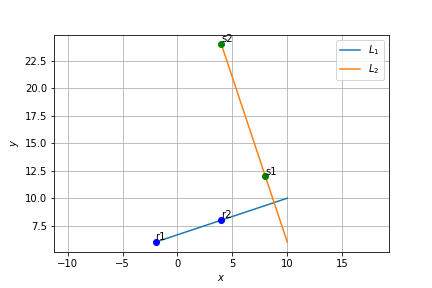
\includegraphics[width= \columnwidth]{assignment8.png}
    \caption{Lines $L_1$ and $L_2$}
    \label{fig:1}
\end{figure}

\end{document}

